\chapter{Implementacja systemu}

System został zaimplementowany w języku \textbf{Java}, z wykorzystaniem biblioteki \textbf{Swing} do budowy graficznego interfejsu użytkownika oraz technologii \textbf{JDBC} do komunikacji z bazą danych \textbf{PostgreSQL}.

\section{Struktura aplikacji}

Struktura projektu została logicznie podzielona na pakiety zgodnie z zasadami dobrej organizacji kodu. W folderze \texttt{src} znajdują się wszystkie elementy źródłowe aplikacji, zorganizowane w następujący sposób:

\begin{itemize}
    \item \texttt{dao} – klasy odpowiedzialne za dostęp do danych:
    \begin{itemize}
        \item \texttt{LoginDAO} – obsługa uwierzytelniania użytkownika;
        \item \texttt{ZajeciaDAO} – operacje CRUD na tabeli zajęć.
    \end{itemize}

    \item \texttt{database} – logika połączenia z bazą danych:
    \begin{itemize}
        \item \texttt{DatabaseConnection} – klasa łącząca aplikację z PostgreSQL.
    \end{itemize}

    \item \texttt{DodajZajeciaPanel} – komponent GUI odpowiedzialny za dodawanie nowych zajęć:
    \begin{itemize}
        \item \texttt{DodajZajeciaPanel.java/.form} – panel formularza oraz jego widok.
    \end{itemize}

    \item \texttt{EdytujZajeciaPanel} – komponent GUI służący do edycji zajęć:
    \begin{itemize}
        \item \texttt{EdytujZajeciaPanel.java/.form} – logika i widok edycji.
    \end{itemize}

    \item \texttt{Login} – komponent odpowiedzialny za ekran logowania:
    \begin{itemize}
        \item \texttt{Login.java/.form} – widok i obsługa logowania.
    \end{itemize}

    \item \texttt{model} – klasy reprezentujące dane biznesowe:
    \begin{itemize}
        \item \texttt{Zajecia} – klasa bazowa reprezentująca ogólne zajęcia;
        \item \texttt{Wyklad}, \texttt{Projekt}, \texttt{Laboratorium} – klasy dziedziczące;
        \item \texttt{PlanZajec} – klasa pomocnicza reprezentująca pojedynczy wpis w planie.
    \end{itemize}

    \item \texttt{SekretariatPanel} – główny interfejs do zarządzania zajęciami:
    \begin{itemize}
        \item \texttt{SekretariatPanel.java/.form} – widok panelu oraz jego logika.
    \end{itemize}

    \item \texttt{resourse} – folder przechowujący zasoby zewnętrzne (np. ikony lub grafiki).

    \item \texttt{Main.java} – klasa uruchamiająca aplikację.
\end{itemize}

Takie rozdzielenie pozwala na lepszą czytelność kodu, łatwiejsze zarządzanie komponentami oraz zgodność z zasadami programowania obiektowego.

\chapter{Harmonogram realizacji projektu}

W poniższej tabeli oraz na wykresie Gantta przedstawiono plan realizacji projektu wraz z zakładanym czasem trwania każdego etapu.

\begin{figure}[H]
    \centering
    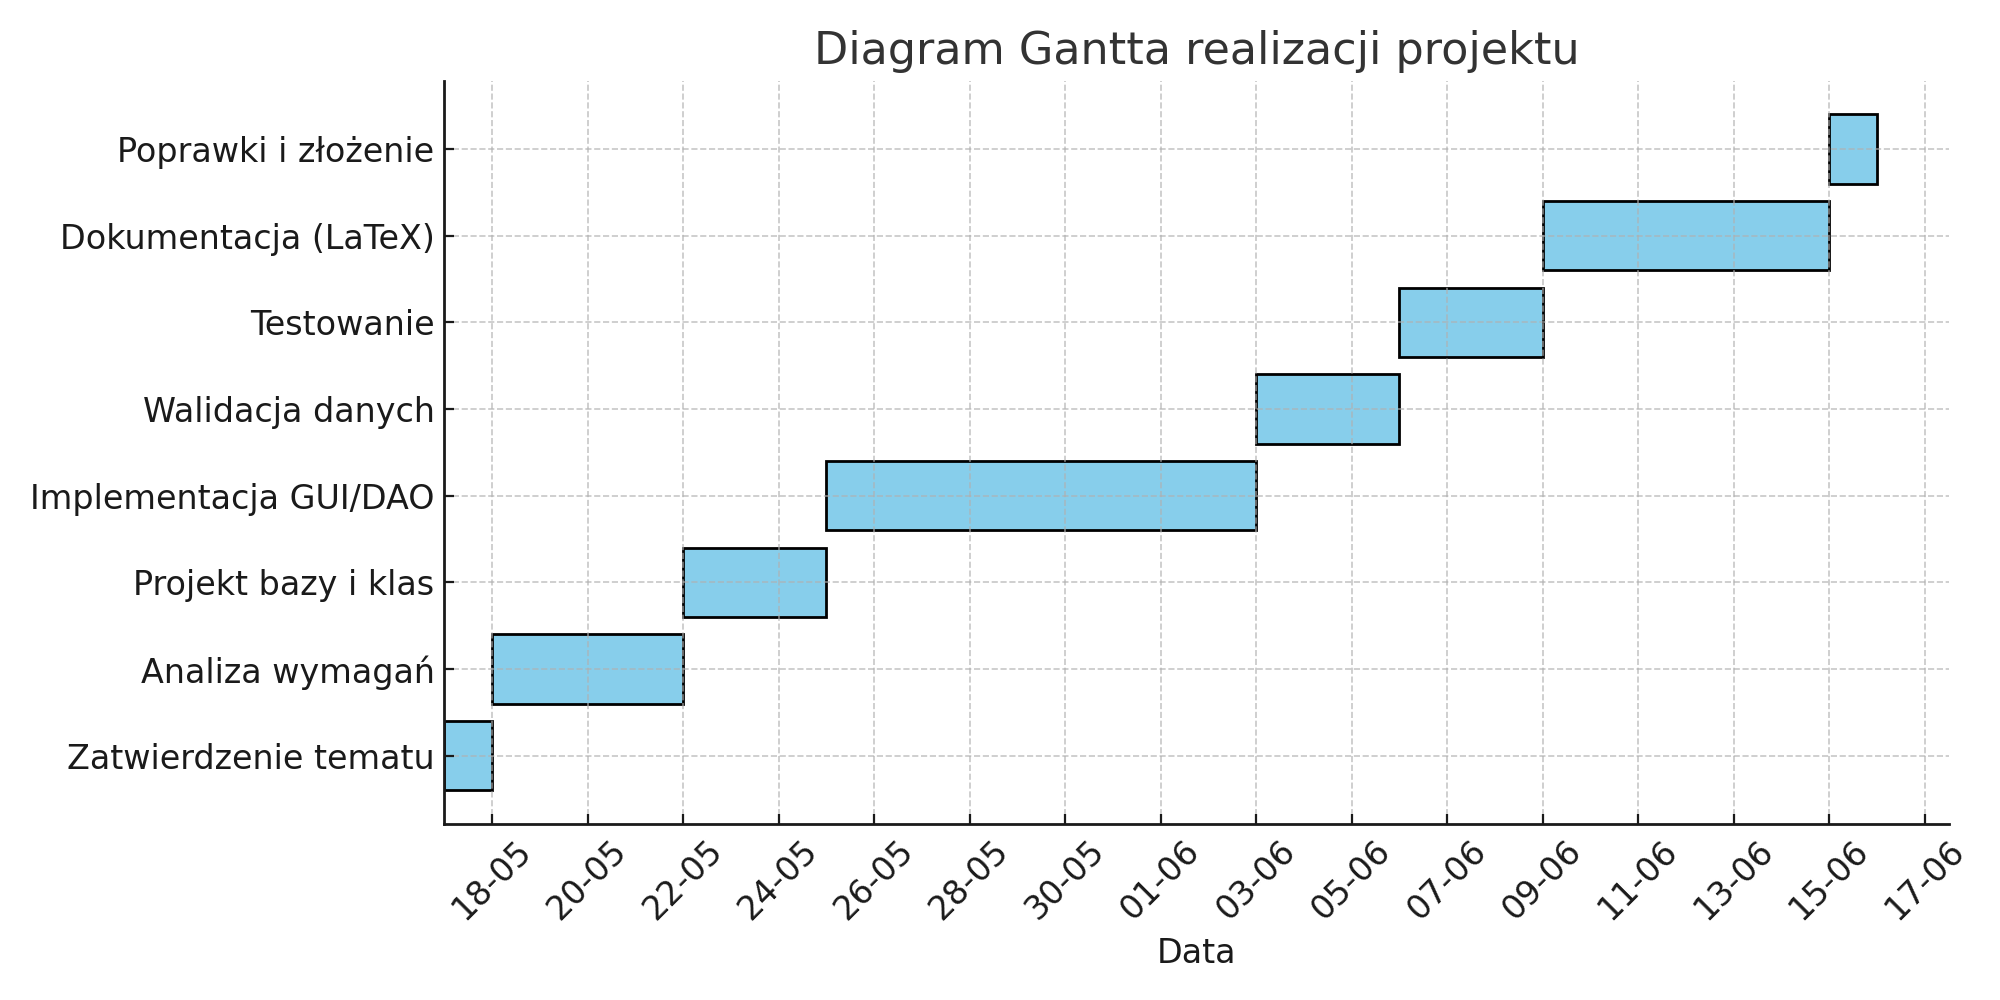
\includegraphics[width=\textwidth]{figures/diagram_gantta_colored_fixed.png}
    \caption{Harmonogram realizacji projektu w formie wykresu Gantta}
    \label{fig:gantt_diagram}
\end{figure}
